\pdfbookmark{Общая характеристика работы}{characteristic}             % Закладка pdf
\section*{Общая характеристика работы}

\newcommand{\actuality}{\pdfbookmark[1]{Актуальность}{actuality}\textbf{\actualityTXT}}
\newcommand{\speciality}{\pdfbookmark[1]{Область исследования}{speciality}\textbf{\specialityTXT}}
\newcommand{\progress}{\pdfbookmark[1]{Разработанность темы}{progress}\textbf{\progressTXT}}
\newcommand{\aim}{\pdfbookmark[1]{Цели}{aim}{\textbf\aimTXT}}
\newcommand{\object}{\pdfbookmark[1]{Объектом исследования}{object}\textbf{\objectTXT}}
\newcommand{\objective}{\pdfbookmark[1]{Предметом исследования}{objective}\textbf{\objectiveTXT}}
\newcommand{\tasks}{\pdfbookmark[1]{Задачи}{tasks}\textbf{\tasksTXT}}
\newcommand{\aimtasks}{\pdfbookmark[1]{Цели и задачи}{aimtasks}\aimtasksTXT}
\newcommand{\novelty}{\pdfbookmark[1]{Научная новизна}{novelty}\textbf{\noveltyTXT}}
\newcommand{\influence}{\pdfbookmark[1]{Практическая значимость}{influence}\textbf{\influenceTXT}}
\newcommand{\methods}{\pdfbookmark[1]{Методология и методы исследования}{methods}\textbf{\methodsTXT}}
\newcommand{\defpositions}{\pdfbookmark[1]{Положения, выносимые на защиту}{defpositions}\textbf{\defpositionsTXT}}
\newcommand{\reliability}{\pdfbookmark[1]{Достоверность}{reliability}\textbf{\reliabilityTXT}}
\newcommand{\probation}{\pdfbookmark[1]{Апробация}{probation}\textbf{\probationTXT}}
\newcommand{\contribution}{\pdfbookmark[1]{Личный вклад}{contribution}\textbf{\contributionTXT}}
\newcommand{\publications}{\pdfbookmark[1]{Публикации}{publications}\textbf{\publicationsTXT}}


%Обзор, введение в тему, обозначение места данной работы в
%мировых исследованиях и~т.\:п., можно использовать ссылки на~другие
%работы~\autocite{Gosele1999161,Lermontov}
%(если их~нет, то~в~автореферате
%автоматически пропадёт раздел <<Список литературы>>). Внимание! Ссылки
%на~другие работы в~разделе общей характеристики работы можно
%использовать только при использовании \verb!biblatex! (из-за технических
%ограничений \verb!bibtex8!. Это связано с тем, что одна
%и~та~же~характеристика используются и~в~тексте диссертации, и в
%автореферате. В~последнем, согласно ГОСТ, должен присутствовать список
%работ автора по~теме диссертации, а~\verb!bibtex8! не~умеет выводить в~одном
%файле два списка литературы).
%При использовании \verb!biblatex! возможно использование исключительно
%в~автореферате подстрочных ссылок
%для других работ командой \verb!\autocite!, а~также цитирование
%собственных работ командой \verb!\cite!. Для этого в~файле
%\verb!common/setup.tex! необходимо присвоить положительное значение
%счётчику \verb!\setcounter{usefootcite}{1}!.
%Настроить размер изображения с логотипом можно
%в~соответствующих местах файлов \verb!title.tex!  отдельно для
%диссертации и автореферата. Если вам логотип не~нужен, то просто
%удалите файл с~логотипом.

%\ifsynopsis
%Этот абзац появляется только в~автореферате.
%Для формирования блоков, которые будут обрабатываться только в~автореферате,
%заведена проверка условия \verb!\!\verb!ifsynopsis!.
%Значение условия задаётся в~основном файле документа (\verb!synopsis.tex! для
%автореферата).
%\else
%Этот абзац появляется только в~диссертации.
%Через проверку условия \verb!\!\verb!ifsynopsis!, задаваемого в~основном файле
%документа (\verb!dissertation.tex! для диссертации), можно сделать новую
%команду, обеспечивающую появление цитаты в~диссертации, но~не~в~автореферате.
%\fi

%В папке Documents можно ознакомиться в решением совета из Томского ГУ
%в~файле \verb+Def_positions.pdf+, где обоснованно даются рекомендации
%по~формулировкам защищаемых положений.


{\actuality} Системы идентификации автомобилей и регистрации нарушений правил дорожного движения играют важную роль в управлении безопасностью на дорогах, способствуют повышению неотвратимости наказания и снижению смертности в авариях. Существующие системы основаны на видео- или фото-идентификации номеров автомобилей. Работе этих систем могут препятствовать загрязнение при плохих погодных условиях или намеренное скрытие номерного знака. Из-за этого, по сведениям ГИБДД, эффективность систем идентификации автомобилей может падать ниже 50~\%. Это определяет актуальность тематики диссертации, направленной на исследование и создание новых систем безопасности, использующих альтернативные источники идентификации транспортных средств, а именно "--- технологию радиочастотной идентификации (RFID). Постановлением Правительства РФ предусмотрено создание в 2022 -- 2024 гг. таких систем в пилотных зонах в Москве, Санкт-Петербурге и Казани.

При использовании RFID-технологии в номерной знак или под лобовое стекло автомобиля помещается радиометка, которая, находясь в области действия RFID-считывателя, передает ему свой идентификатор. В пассивных системах RFID УВЧ-диапазона 860 -- 960~МГц метки не обладают собственными источниками энергии и могут быть идентифицированы считывателями на расстоянии порядка 10 -- 20 метров. Эффективность радиочастотной идентификации существенно зависит как от особенностей окружения, распространения радиосигналов и антенн, так и от параметров протокола связи между считывателем и метками международного стандарта EPC Class 1 Generation 2 (EPC Gen2). Хотя анализу производительности систем радиочастотной идентификации в различных приложениях посвящено немало работ, тема применения RFID для идентификации автомобилей остается менее изученной с теоретической точки зрения. Для получения адекватной оценки производительности в диссертации предложены и исследованы новые математические и имитационные модели, учитывающие как параметры распространения радиосигналов, так и всевозможные настройки считывателей и параметры протокола.

Для работы автоматической системы безопасности необходимо соединять точки идентификации с центрами обработки данных компьютерными сетями, по которым оперативно передается информация о распознанных автомобилях. Проводные решения оказываются не всегда доступными по техническим или экономическим причинам, поэтому особый интерес представляют беспроводные сети. Для анализа проивзодительности беспроводных сетей часто применяются стохастические методы, но из-за высокой сложности их зачастую трудно применять для анализа больших многошаговых сетей. Одним из наиболее распространённых методов исследований являются сети массового обслуживания (СеМО), в которых каналы связи и маршрутизаторы моделируются обслуживающими приборами с очередями. Хорошую точность при описании реальных систем показывают СеМО с марковсиким входящими потоками (MAP) и распределением времени обслуживания фазового типа (PH). Хотя системы MAP/PH/1/N хорошо исследованы, их применение для построения открытых сетей массового обслуживания, моделирующих реальные беспроводные сети, мало изучено в современной литературе. Из-за высокой сложности моделей особый интерес представляют методы быстрого получения приближенных оценок их характеристик, разработанные в настоящей работе.

Системы управления RFID-считывателями, используемые в системах безопасности на автодорогах, обладают рядом особенностей. Во-первых, они должны обеспечивать непрерывный сбор данных с большого количества RFID-считывателей в реальном времени. Во-вторых, необходимо объединять данные о прочитанных RFID-метках с данными от камер видеофиксации, радарами и другими датчиками. Наконец, для различных служб и ведомств система должна предоставлять разные уровени доступа. Перечисленные особенности делают актуальной задачу разработки новой распределенной системы управления считывателями, предложенной в диссертационной работе.
% Для реализации системы радиочастотной идентификации транспорта нужны системы управления и программное обеспечение для связи считывателей с центрами обработки данных,

Таким образом, высокая практическая потребность в разработке новых систем управления безопасностью дорожного движения на основе RFID-технологии и широкополосной беспроводной связи определяет актуальность и новизну диссертационной работы.

Исследованиям в области разработки и исследования широкополосных беспроводных сетей и технологии RFID, методам теории массового обслуживания и вопросам ее применения и прочим темам, затрагиваемым в диссертации, посвящен ряд работ, среди которых следует особо отметить работы отечественных и зарубежных учёных: В.М. Вишневский, А.Н. Дудин, П.В. Никитин, А.Е. Кучерявый, К.Е. Самуйлов, Ю.В. Гайдамака, В.В. Рыков, Р.Н. Минниханов, D. Lucantoni, N. Abramson, L.G. Roberts, M.F. Neuts, G. Horvath, G. Bianchi,  H. Okamura, P. Buchholz, M. Telek, J.C. Strelen, L. Bodrog, D. Aldous, K.V.S. Rao, C. Floerkemeier, C. Wang, E. Vahedi, R. Nelson, T.S. Rappaport, S. Singh, J. Kriege, P. Djukic, S. Valaee, J.E. Hoag. и др.

% {\progress}
% Этот раздел должен быть отдельным структурным элементом по
% ГОСТ, но он, как правило, включается в описание актуальности
% темы. Нужен он отдельным структурынм элемементом или нет ---
% смотрите другие диссертации вашего совета, скорее всего не нужен.

{\object} являются системы радиочастотной идентификации транспорта и опорные многошаговые беспроводные сети. {\objective} являются методы анализа и алгоритмы расчета характеристик производительности систем радиочастотной идентификации и многошаговых беспроводных сетей, а также методы построения систем управления распределенными системами идентификации транспорта.

{\aim} данной работы является создание комплекса моделей для анализа производительности систем радиочастотной идентификации и широкополосных беспроводных сетей, а также разработка и экспериментальное внедрение системы управления и сбора данных с RFID-считывателей.

Для~достижения поставленной цели было необходимо решить следующие {\tasks}:
\begin{enumerate}[beginpenalty=10000] % https://tex.stackexchange.com/a/476052/104425
  \item Разработать комплекс аналитических и имитационных моделей для анализа производительности систем радиочастотной идентификации транспортных средств, позволяющих адекватно оценивать их производительность.
  \item Разработать комплекс аналитических моделей на базе методов теории массового обслуживания для оценки производительности опорных беспроводных сетей с использованием марковских случайных потоков для моделирования трафика и распределений фазового типа для моделирования процесса передачи данных, а также методов понижения размерности для нахождения эффективных способов расчёта показателей производительности.
  \item Разработать распределенную систему управления и сбора данных с RFID-считывателей и провести её экспериментальное внедрение.
\end{enumerate}


{\novelty}
\begin{enumerate}[beginpenalty=10000] % https://tex.stackexchange.com/a/476052/104425
  \item Впервые предложена стохастическая модель системы радиочастотной идентификации с мобильными метками, учитывающая различные законы движения меток, а также сценарии переключения питания и смены опрашиваемых значений флагов сессий.
  \item Предложен комплекс новых аналитических и имитационных моделей для анализа вероятности идентификации быстро движущихся транспортных средств с учетом особенностей логического и физического уровней EPC Gen2, а также учитывающих особенности распространения радиосигналов вблизи автодороги.
  \item Предложена новая методика построения сетей массового обслуживания с марковскими входными потоками и распределениями фазового типа для адекватного моделирования многошаговых беспроводных сетей, учитывающая различия в трафике и интерференции, испытываемые разными станциями сети.
  \item Предложен и исследован метод приближенного вычисления оценок характеристик тандемных открытых сетей массового обслуживания с коррелированными марковскими входными потоками и распределениями обслуживания фазового типа, основанный на аппроксимации потоков обслуженных заявок PH-распределениями или MAP-потоками по первым моментам и автокорреляции. В численном эксперименте показано, что предложенный метод позволяет находить оценки характеристик сети с высокой точностью за малое время.
  \item Разработана и реализована новая распределенная система управления RFID-считывателями, предназначенная для организации сбора данных об идентифицированных транспортных средствах и допускающая объединение с данными, поступающими от прочих источников идентификации.
  \item Проведено три эксперимента по внедрению системы радиочастотной идентификации на дорогах в г. Казань и на ЦКАД в Московской области, получены экспериментальные данные об эффективности разработанной системы.
\end{enumerate}

{\speciality}
Диссертационная работа соответствует содержанию специальности 05.13.15, а именно исследованиям и разработке научных основ архитектурных, структурных, логических и технических принципов создания вычислительных машин, комплексов и компьютерных сетей, организации арифметической, логической, символьной и специальной обработки данных, хранения и ввода-вывода информации, параллельной и распределенной обработки информации, многопроцессорных и многомашинных вычислительных систем, сетевых протоколов и служб передачи данных в компьютерных сетях, взаимодействия и защиты компьютерных сетей. В выполненной работе
присутствуют оригинальные результаты одновременно из четырех областей: разработка принципов создания компьютерных сетей, математического моделирования копмьютерных сетей, численных методов и комплексов программ. Диссертационная работа соответствует следующим пунктам специальности:
\begin{itemize}
    \item Разработка научных основ создания вычислительных машин, комплексов и компьютерных сетей, исследования общих свойств и принципов функционирования вычислительных машин, комплексов и компьютерных сетей.
    \item Теоретический анализ и экспериментальное исследование функционирования вычислительных машин, комплексов и компьютерных сетей с целью улучшения их технико-экономических и эксплуатационных характеристик.
    \item Разработка научных методов и алгоритмов организации параллельной и распределенной обработки информации, многопроцессорных, многомашинных и специальных вычислительных систем.
    \item Разработка научных методов и алгоритмов создания структур и топологий компьютерных сетей, сетевых протоколов и служб передачи данных в компьютерных сетях, взаимодействия компьютерных сетей, построенных с использованием различных телекоммуникационных технологий, мобильных и специальных компьютерных сетей, защиты компьютерных сетей и приложений.
\end{itemize}

{\influence}
Аналитические модели протокола EPC Gen2, предложенные в работе, могут использоваться для первоначальной оценки производительности системы радиочастотной идентификации автомобилей. Имитационная модель этой системы, учитывающая особенности протокола, оборудования и канала связи между считывателем и метками, может использоваться для получения оценок производительности системы при различных интенсивностях и скоростях дорожного движения.

Модели многошаговых беспроводных сетей могут использоваться для оценки производительности (межконцевых задержек и вероятностей потери пакетов) при проектировании телекоммуникационных сетей.

Распределенная система управления считывателями и промежуточное программное обеспечение, описанные в работе, использовались в трех экспериментальных внедрениях. Предложенные решения могут использоваться при дальнейшем практическом внедрении системы радиочастотной идентификации автомобилей.

Результаты работы также были использованы в исследованиях, проводимых по следующим грантам:

\begin{itemize}
    \item Контракт c Министерством образования и науки РФ № 14.514.11.4071 в рамках федеральной целевой программы <<Исследования и разработки по приоритетным направлениям развития научно-технологического комплекса России на 2007-2013 годы>>.
	\item Соглашение с Министерством образования и науки РФ о предоставлении субсидии от 22.10.2014 г. № 14.613.21.0020 в рамках федеральной целевой программы <<Исследования и разработки по приоритетным направлениям развития научно-технологического комплекса на 2014-2020 годы>>.
	\item Грант Российского научного фонда (РНФ) № 16-49-02021.
	\item Грант Российского фонда фундаментальных исследований (РФФИ) № 13-07-00737.
	\item Грант Российского фонда фундаментальных исследований (международный проект РФФИ "--- БРФФИ) № 14-07-90015.
	\item Грант Российского фонда фундаментальных исследований (международный проект РФФИ "--- БРФФИ) № 16-57-00130.

	% \item Контракт c Министерством образования и науки РФ № 14.514.11.4071 в рамках федеральной целевой программы <<Исследования и разработки по приоритетным направлениям развития научно-технологического комплекса России на 2007-2013 годы>> поисковые научно-исследовательские работы по лоту шифр <<2013-1.4-14-514-0122>> <<Разработка технологии и архитектуры аппаратно-программных средств сверхвысокоскоростных беспроводных сетей в миллиметровом диапазоне радиоволн 60-100 ГГц>> по теме: <<Разработка и исследование технологии и архитектуры сверхвысокоскоростных беспроводных сетей в миллиметровом Е-диапазоне радиоволн 71-76 ГГц, 81-86 ГГц>>
	% \item Соглашение с Министерством образования и науки РФ о предоставлении субсидии от 22.10.2014 г. № 14.613.21.0020 в рамках федеральной целевой программы <<Исследования и разработки по приоритетным направлениям развития научно-технологического комплекса на 2014-2020 годы>> по теме: <<Разработка математических методов, алгоритмов и программ оценки производительности и проектирования широкополосных беспроводных сетей передачи мультимедийной информации вдоль протяженных транспортных магистралей (железнодорожное полотно, автодороги) и трубопроводов (нефтяные и газовые магистрали)>>
	% \item Грант Российского научного фонда (РНФ) № 16-49-02021 <<Новый комплекс математических моделей, методов, алгоритмов и программ управляемых стохастических систем для оценки производительности и проектирования телекоммуникационных сетей следующего поколения>>
	% \item Грант Российского фонда фундаментальных исследований (РФФИ) № 13-07-00737 <<Разработка принципов построения и математических методов исследования нового класса автоматизированных систем безопасности на автодорогах с использованием RFID-технологий и высокоскоростной беспроводной связи>>
	% \item Грант Российского фонда фундаментальных исследований (международный проект РФФИ "--- БРФФИ) № 14-07-90015 Бел\_а <<Разработка и исследование методов оценки производительности и проектирования гибридных систем передачи мультимедийной информации на базе лазерной и радио технологий>>
	% \item Грант Российского фонда фундаментальных исследований (международный проект РФФИ "--- БРФФИ) № 16-57-00130 Бел\_а <<Разработка и исследование методов синтеза архитектуры широкополосных беспроводных сетей с линейной топологией>>
\end{itemize}

{\methods} Для решения задач, поставленных в диссертации, использовались методы теории вероятности, математической статистики, теории случайных процессов, теории массового обслуживания, методы моделирования беспроводных протоколов и сетей с помощью марковских цепей, методы дискретно-событийного имитационного моделирования. При разработке программного обеспечения использовались методоы многопоточного программирования, методы разработки распределенных систем.

{\defpositions}
\begin{enumerate}[beginpenalty=10000] % https://tex.stackexchange.com/a/476052/104425
  \item Стохастическая модель системы радиочастотной идентификации с мобильными метками, учитывающая различные законы движения меток, а также сценарии переключения питания и смены опрашиваемых значений флагов сессий.
  \item Комплекс аналитических и имитационных моделей для анализа вероятности идентификации быстро движущихся транспортных средств с учетом особенностей логического и физического уровней EPC Gen2, а также особенностей распространения радиосигналов вблизи автодороги.
  \item Метод построения моделей открытых тандемных сетей массового обслуживания для анализа производительности многошаговых беспроводных сетей.
  \item Метод расчета оценок характеристик открытых сетей массового обслуживания с марковскими входящими потоками и обслуживанием фазового типа с использованием аппроксимации потоков обслуженных пакетов PH-распределениями и MAP-потоками.
  \item Реализация распределенной системы управления RFID-считывателями, используемой для создания систем радиочастотной идентификации автотранспорта.
\end{enumerate}

{\reliability} полученных результатов обеспечивается использованием строгих математических моделей, сравнением результатов аналитического и имитационного моделирования. Результаты анализа вероятности идентификации автомобилей согласуются с результатами, полученными в ходе реальных экспериментов. Результаты находятся в соответствии с результатами, полученными другими авторами.


{\probation}
Основные результаты работы докладывались~на следующих конференциях: 12th Annual IEEE International conference on RFID 2018 (IEEE RFID 2018; США, Орландо); 11th Annual IEEE International conference on RFID 2017 (IEEE RFID 2017; США, Финикс); международный форум Kazan Digital Week 2020 (Казань); International conference on Advances in Applied Probability and Stochastic Processes 2019 (ICAAP \& SP 2019; Индия, Коттаям); 13-е и 12-е Всероссийские совещания по проблемам управления (ВСПУ 2019, ВСПУ 2014; Москва, ИПУ РАН); 20-я, 18-я, 16-я и 15-я Международные конференции им. А.Ф. Терпугова Информационные технологии и математическое моделирование (ИТММ 2021, ИТММ 2019, ИТММ 2017, ИТММ 2016; Россия); 11th IEEE International Conference on Application of Information and Communication Technologies (IEEE AICT 2017; Москва, ИПУ РАН); 21-я, 20-я, 19-я, 18-я и 17-я Международные Конференции <<Распределенные компьютерные и телекоммуникационные сети: управление, вычисление, связь>> (DCCN 2018, DCCN 2017, DCCN 2016, DCCN 2015, DCCN 2013; Москва); 7th International Workshop on Communication Technologies for Vehicles (Nets4Cars-Fall 2014; Санкт-Петербург); 2012 International Conference on RFID-Technology and Applications (IEEE RFID-TA 2012; Франция, Ницца); 10-я и 5-я Всероссийская конференция <<Информационно-телекоммуникационные технологии и математическое моделирование высокотехнологичных систем>> (ИТТММ 2020, ИТТММ 2015; Москва, РУДН).

{\contribution} Автор принимал активное участие в разработке стохастической модели протокола EPC Gen2, имитационной модели системы радиочастотной идентификации автомобилей, аналитической и имитационной модели для расчёта производительности многошаговых беспроводных сетей, методов расчета характеристик тандемных сетей массового обслуживания, промежуточного программного обеспечения и системы управления считывателями, разработке считывателя и проведении экспериментов.

\ifnumequal{\value{bibliosel}}{0}
{%%% Встроенная реализация с загрузкой файла через движок bibtex8. (При желании, внутри можно использовать обычные ссылки, наподобие `\cite{vakbib1,vakbib2}`).
    {\publications} Основные результаты по теме диссертации изложены
    в~XX~печатных изданиях,
    X из которых изданы в журналах, рекомендованных ВАК,
    X "--- в тезисах докладов.
}%
{%%% Реализация пакетом biblatex через движок biber
    \begin{refsection}[bl-author, bl-registered]
        % Это refsection=1.
        % Процитированные здесь работы:
        %  * подсчитываются, для автоматического составления фразы "Основные результаты ..."
        %  * попадают в авторскую библиографию, при usefootcite==0 и стиле `\insertbiblioauthor` или `\insertbiblioauthorgrouped`
        %  * нумеруются там в зависимости от порядка команд `\printbibliography` в этом разделе.
        %  * при использовании `\insertbiblioauthorgrouped`, порядок команд `\printbibliography` в нём должен быть тем же (см. biblio/biblatex.tex)
        %
        % Невидимый библиографический список для подсчёта количества публикаций:
        \printbibliography[heading=nobibheading, section=1, env=countauthorvak,          keyword=biblioauthorvak]%
        \printbibliography[heading=nobibheading, section=1, env=countauthorwos,          keyword=biblioauthorwos]%
        \printbibliography[heading=nobibheading, section=1, env=countauthorscopus,       keyword=biblioauthorscopus]%
        \printbibliography[heading=nobibheading, section=1, env=countauthorconf,         keyword=biblioauthorconf]%
        \printbibliography[heading=nobibheading, section=1, env=countauthorother,        keyword=biblioauthorother]%
        \printbibliography[heading=nobibheading, section=1, env=countregistered,         keyword=biblioregistered]%
        \printbibliography[heading=nobibheading, section=1, env=countauthorpatent,       keyword=biblioauthorpatent]%
        \printbibliography[heading=nobibheading, section=1, env=countauthorprogram,      keyword=biblioauthorprogram]%
        \printbibliography[heading=nobibheading, section=1, env=countauthor,             keyword=biblioauthor]%
        \printbibliography[heading=nobibheading, section=1, env=countauthorvakscopuswos, filter=vakscopuswos]%
        \printbibliography[heading=nobibheading, section=1, env=countauthorscopuswos,    filter=scopuswos]%
        %
        \nocite{*}%
        %
        {\publications} Основные результаты по теме диссертации изложены в~\arabic{citeauthor}~печатных изданиях,
        \arabic{citeauthorvak} из которых изданы в журналах, рекомендованных ВАК\sloppy%
        \ifnum \value{citeauthorscopuswos}>0%
            , \arabic{citeauthorscopuswos} "--- в~изданиях, индексируемых Web of~Science и Scopus\sloppy%
        \fi%
        \ifnum \value{citeauthorconf}>0%
            , \arabic{citeauthorconf} "--- в~тезисах докладов.
        \else%
            .
        \fi%
        \ifnum \value{citeregistered}=1%
            \ifnum \value{citeauthorpatent}=1%
                Зарегистрирован \arabic{citeauthorpatent} патент.
            \fi%
            \ifnum \value{citeauthorprogram}=1%
                Зарегистрирована \arabic{citeauthorprogram} программа для ЭВМ.
            \fi%
        \fi%
        \ifnum \value{citeregistered}>1%
            Зарегистрированы\ %
            \ifnum \value{citeauthorpatent}>0%
            \formbytotal{citeauthorpatent}{патент}{}{а}{}\sloppy%
            \ifnum \value{citeauthorprogram}=0 . \else \ и~\fi%
            \fi%
            \ifnum \value{citeauthorprogram}>0%
            \formbytotal{citeauthorprogram}{программ}{а}{ы}{} для ЭВМ.
            \fi%
        \fi%
        % К публикациям, в которых излагаются основные научные результаты диссертации на соискание учёной
        % степени, в рецензируемых изданиях приравниваются патенты на изобретения, патенты (свидетельства) на
        % полезную модель, патенты на промышленный образец, патенты на селекционные достижения, свидетельства
        % на программу для электронных вычислительных машин, базу данных, топологию интегральных микросхем,
        % зарегистрированные в установленном порядке.(в ред. Постановления Правительства РФ от 21.04.2016 N 335)
    \end{refsection}%
    \begin{refsection}[bl-author, bl-registered]
        % Это refsection=2.
        % Процитированные здесь работы:
        %  * попадают в авторскую библиографию, при usefootcite==0 и стиле `\insertbiblioauthorimportant`.
        %  * ни на что не влияют в противном случае
        \nocite{RFID_JRFID2017}
        \nocite{WINET_IJPAM2016}
        \nocite{WINET_TCOMM2015}
        \nocite{QS_JPU2013}
        \nocite{QS_JITCS2013}
        \nocite{QS_TCOMM2012}

        \nocite{QS_ICAAPSP2020}
        \nocite{QS_ITMM2019}
        \nocite{RFID_IEEERFID2018}
        \nocite{RFID_SYNCHROINFO2018}
        \nocite{RFID_IEEERFID2017}
        \nocite{QS_AICT2017}
        \nocite{QS_ITMM2017}
        \nocite{QS_ITMM2016}
        \nocite{QS_DCCN2016_CCIS}
        \nocite{RFID_DCCN2016_CCIS}
        \nocite{RFIDCTRL_NETS2CARS2014}
        \nocite{RFIDTA2012}

        % \nocite{vakbib2}%vak
        % \nocite{patbib1}%patent
        % \nocite{progbib1}%program
        % \nocite{bib1}%other
        % \nocite{confbib1}%conf
    \end{refsection}%
        %
        % Всё, что вне этих двух refsection, это refsection=0,
        %  * для диссертации - это нормальные ссылки, попадающие в обычную библиографию
        %  * для автореферата:
        %     * при usefootcite==0, ссылка корректно сработает только для источника из `external.bib`. Для своих работ --- напечатает "[0]" (и даже Warning не вылезет).
        %     * при usefootcite==1, ссылка сработает нормально. В авторской библиографии будут только процитированные в refsection=0 работы.
}

% При использовании пакета \verb!biblatex! будут подсчитаны все работы, добавленные
% в файл \verb!biblio/author.bib!. Для правильного подсчёта работ в~различных
% системах цитирования требуется использовать поля:
% \begin{itemize}
%         \item \texttt{authorvak} если публикация индексирована ВАК,
%         \item \texttt{authorscopus} если публикация индексирована Scopus,
%         \item \texttt{authorwos} если публикация индексирована Web of Science,
%         \item \texttt{authorconf} для докладов конференций,
%         \item \texttt{authorpatent} для патентов,
%         \item \texttt{authorprogram} для зарегистрированных программ для ЭВМ,
%         \item \texttt{authorother} для других публикаций.
% \end{itemize}
% Для подсчёта используются счётчики:
% \begin{itemize}
%         \item \texttt{citeauthorvak} для работ, индексируемых ВАК,
%         \item \texttt{citeauthorscopus} для работ, индексируемых Scopus,
%         \item \texttt{citeauthorwos} для работ, индексируемых Web of Science,
%         \item \texttt{citeauthorvakscopuswos} для работ, индексируемых одной из трёх баз,
%         \item \texttt{citeauthorscopuswos} для работ, индексируемых Scopus или Web of~Science,
%         \item \texttt{citeauthorconf} для докладов на конференциях,
%         \item \texttt{citeauthorother} для остальных работ,
%         \item \texttt{citeauthorpatent} для патентов,
%         \item \texttt{citeauthorprogram} для зарегистрированных программ для ЭВМ,
%         \item \texttt{citeauthor} для суммарного количества работ.
% \end{itemize}
% % Счётчик \texttt{citeexternal} используется для подсчёта процитированных публикаций;
% % \texttt{citeregistered} "--- для подсчёта суммарного количества патентов и программ для ЭВМ.

% Для добавления в список публикаций автора работ, которые не были процитированы в
% автореферате, требуется их~перечислить с использованием команды \verb!\nocite! в
% \verb!Synopsis/content.tex!. % Характеристика работы по структуре во введении и в автореферате не отличается (ГОСТ Р 7.0.11, пункты 5.3.1 и 9.2.1), потому её загружаем из одного и того же внешнего файла, предварительно задав форму выделения некоторым параметрам

%Диссертационная работа была выполнена при поддержке грантов \dots

%\underline{\textbf{Объем и структура работы.}} Диссертация состоит из~введения,
%четырех глав, заключения и~приложения. Полный объем диссертации
%\textbf{ХХХ}~страниц текста с~\textbf{ХХ}~рисунками и~5~таблицами. Список
%литературы содержит \textbf{ХХX}~наименование.

\pdfbookmark{Содержание работы}{description}                          % Закладка pdf
\section*{Содержание работы}
Во \textbf{введении} обосновывается актуальность исследований, проводимых в~рамках данной диссертационной работы, формулируется цель, ставятся задачи работы, излагается научная новизна и практическая значимость представляемой работы, приводится краткое содержание разделов диссертационной работы.


%------------------------------------------------------------------------------
% ГЛАВА 1 (ВВЕДЕНИЕ)
%------------------------------------------------------------------------------
В \textbf{первой главе} подробно рассматривается структура распределенной системы радиочастотной идентификации транспорта, описываются основные задачи и проблемы, возникающие при ее построении, анализе производительности и поиске способов увеличения эффективности. Приводится краткое описание технологии UHF RFID стандарта EPC Class 1 Generation 2 (ISO 18006-C), а также обзор современных исследований в областях анализа производительности, способов применения и разработки систем радиочастотной идентификации. Дается краткое описание метода доступа DCF в IEEE 802.11 и приводится обзор работ, посвященных исследованию и моделированию задержек в каналах беспроводных сетей. Приводится описание многофазной системы массового обслуживания, которая используется в работе для моделирования многошаговой беспроводной сети, даются определения MAP-потоков и PH-распределений и приводится обзор исследований сетей массового обслуживания с MAP-потоками и PH-распределениями. Приводится краткое описание и обзор методов их восстановления по известным статистическим данным. В конце раздела приводится обзор исследований и стандартов в области разработки систем управления и промежуточного программного обеспечения систем радиочастотной идентификации.

% картинку можно добавить так:
% \begin{figure}[ht]
%     \centerfloat{
%         \hfill
%         \subcaptionbox{\LaTeX}{%
%             \includegraphics[scale=0.27]{latex}}
%         \hfill
%         \subcaptionbox{Knuth}{%
%             \includegraphics[width=0.25\linewidth]{knuth1}}
%         \hfill
%     }
%     \caption{Подпись к картинке.}\label{fig:latex}
% \end{figure}

% Формулы в строку без номера добавляются так:
% \[
%   \lambda_{T_s} = K_x\frac{d{x}}{d{T_s}}, \qquad
%   \lambda_{q_s} = K_x\frac{d{x}}{d{q_s}},
% \]


%------------------------------------------------------------------------------
% ГЛАВА 2 (СИМУЛЯЦИЯ RFID)
%------------------------------------------------------------------------------
\textbf{Вторая глава} посвящена исследованию производительности системы радиочастотной идентификации движущихся автомобилей. Рассматривается два способа идентификации: по значению EPCID метки, и по паре значений EPCID и TID. Автомобиль считается идентифицированным, если хотя бы одна метка была успешно прочитана хотя бы один раз. В \S~1 приводится описание структуры исследуемой системы радиочастотной идентификации.

В \S~2 приводится первое приближение для расчета вероятности успешной идентификации движущейся со скоростью $v$ метки:
\[
P_t = 1 - \left( 1 - (1 - 2^{-Q})^{N_t-1} (1 - p_e)^B \right)^{N_r},
\]
где $2^Q$ "--- число слотов в раунде опроса, $N_t$ "--- среднее число меток, принимающих участие в раунде, $p_e$ "--- средняя вероятность битовой ошибки (BER), $B$ "--- общее число бит в ответах метки, $N_r = L / (v \tau)$ "--- среднее число раундов, в которых успевает принять метка, $L$ "--- средняя длина отрезка дороги, на котором метка получает достаточно энергии, $v$ "--- скорость движения метки, а $\tau$ "--- средняя длительность раунда инвентаризации. Чем выше длительность символов в командах считывателя и ответах метки, тем ниже BER $p_e$ и выше средняя длительность раунда $\tau$. Реальное значение BER $p_e(t)$, как и величина $L$, меняются со временем, так как из-за эффекта Доплера канал оказывается зависимым от времени.

В \S~3 исследуется зависимость максимальной длительности раундов и числа раундов, в которых принимает участие метки, от параметров протокола EPC Gen.2 (Tari, M, Q и другие). Показано, что длительности раундов инвентаризации меняются от 700 микросекунд до 400 миллисекунд в зависимости от настроек протокола. Как следствие, теоретически возможное число раундов, в которых метка может передать свой идентификатор, меняется в зависимости от настроек и скорости движения от 1 до 400.

В \S~4 исследуются затухания прямого и отраженного меткой радиосигналов с использованием двухлучевой модели распространения. При этом учитываются поляризация, диаграммы и коэффициенты усиления антенн, потери при отражении от дороги, потери из-за различных поляризаций, потери на модуляции отраженного сигнала. Из-за эффекта Доплера мощности сигналов и величина BER оказываются сильно зависимыми от времени, прошедшего со включения считывателя. В \S~4 приводятся результаты аналитического расчета величин затухания, BER и мощностей принятых сигналов, а также описываются области, в которых метка получает достаточно энергии для работы.

\begin{figure}[h]
  \centerfloat{
    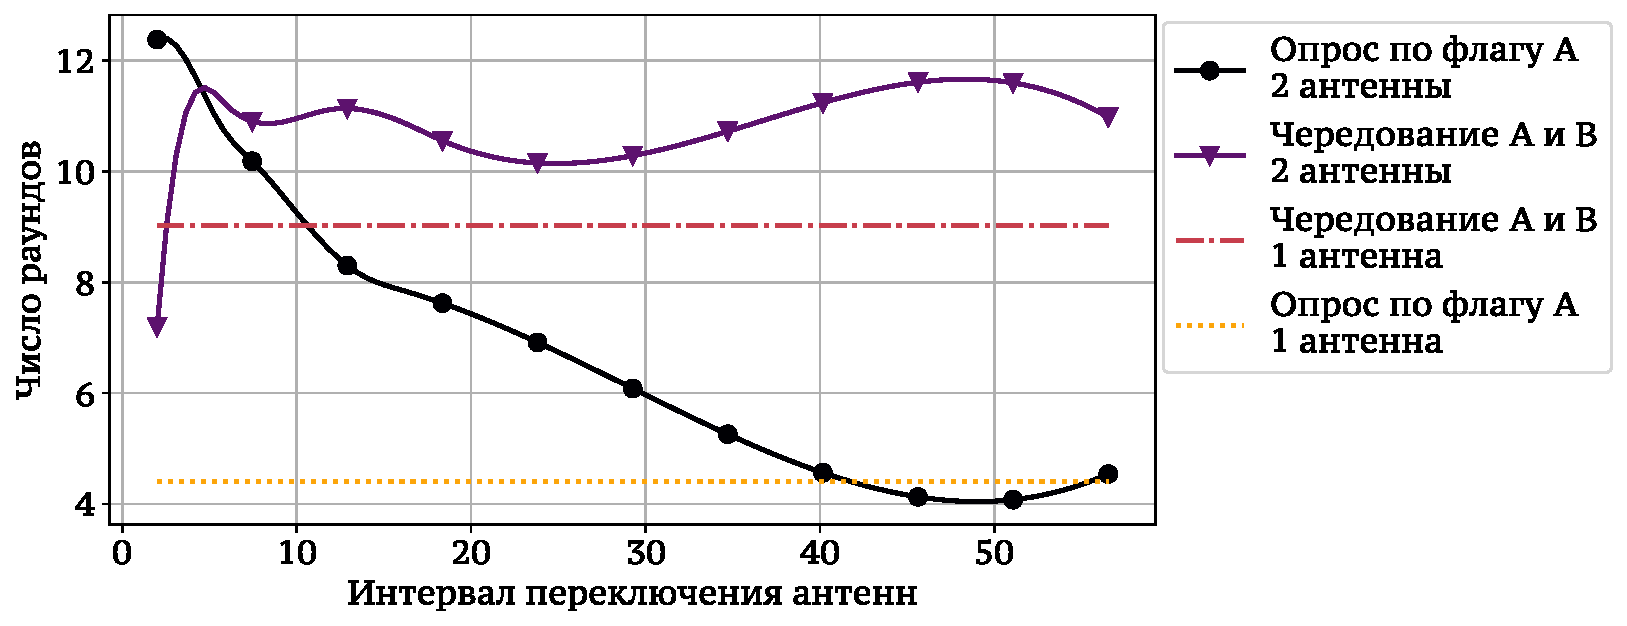
\includegraphics[scale=0.4]{chapter2/ch2_sim_num_rounds_one_lane.pdf}
  }
  \caption{Число раундов, в которых принимает участие метка}\label{fig:rounds_per_tag}
\end{figure}

В \S~5 приводятся численные результаты, полученные с помощью имитационного моделирования. В имитационной модели учитываются форматы всех команд и ответов, с высокой точностью рассчитываются длительности кадров, мощности сигналов, моделируются отключения питания, переключения антенн и смены сессий опроса меток. Сначала приводятся оценки числа раундов $N_r$, в которых успевает принять участие метка (см. рис.~\ref{fig:rounds_per_tag}), в зависимости от частоты переключения антенн и порядка изменений флага сессии в опросе. Затем приводятся результаты расчета вероятности идентификации отдельных меток в передних и задних номерах при различных скоростях движения автомобилей и настройках считывателя. Приводится сравнение результатов, полученных с учетом эффекта Доплера и без него, из которых следует, что этот эффект оказывает существенное влияние на вероятность идентификации, особенно при высоких скоростях движения меток. Также получены результаты расчета вероятности успешной идентификации автомобиля по любой из меток, см. рис.~\ref{fig:vehicle_identification_rate}. Численные эксперименты показывают, что система обладает достаточно высокой эффективностью даже для быстро движущихся автомобилей, когда используются не самые надежные, но и не самые быстрые настройки протокола. При идентификации по EPCID наилучший результат дает использование кода Миллера восьмого порядка (M=8) и Tari = 12,5~мкс, а при идентификации по паре EPCID и TID "--- код Миллера четвертого порядка (M=4) и такое же значение Tari.

\begin{figure}[h]
  \centerfloat{
    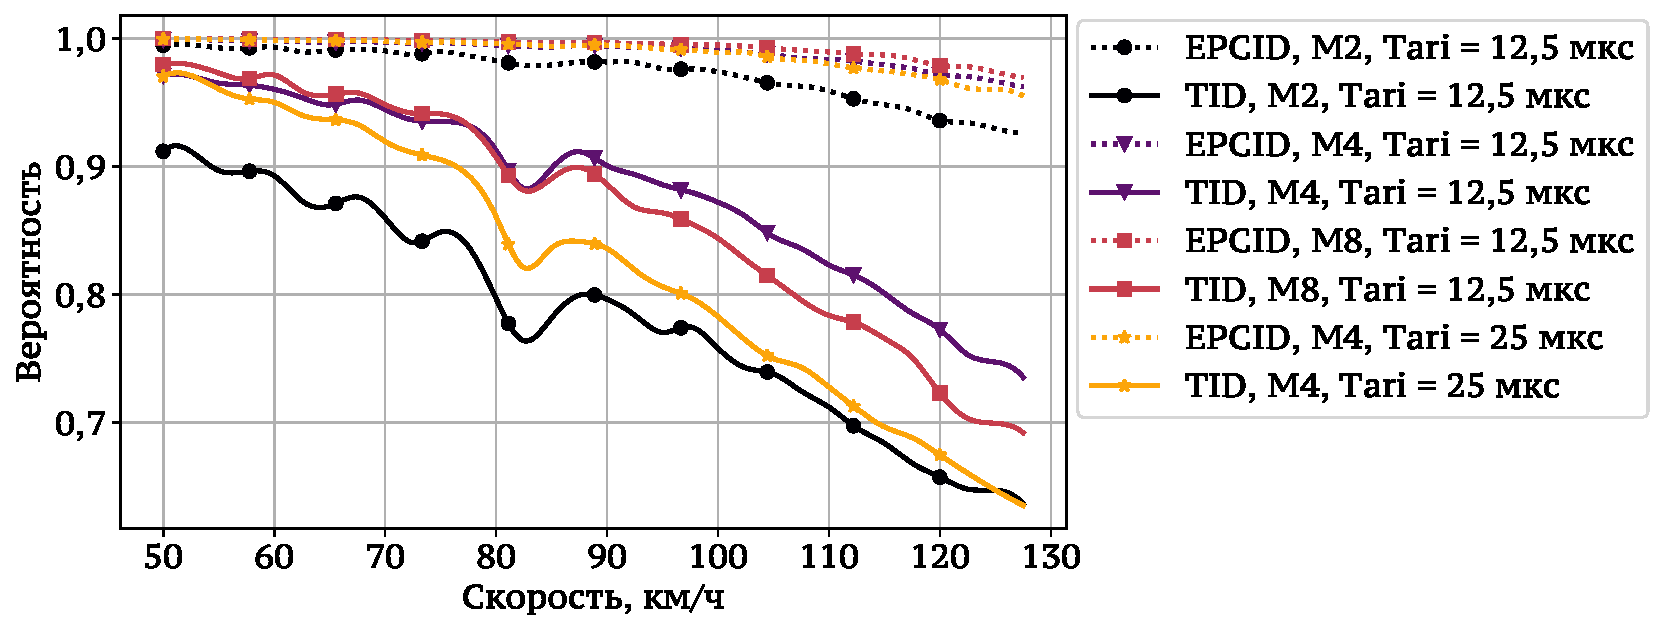
\includegraphics[scale=0.4]{chapter2/ch2_vehicle_identification_rate}
  }
  \caption{Вероятность успешной идентификации автомобиля}\label{fig:vehicle_identification_rate}
\end{figure}




%------------------------------------------------------------------------------
% ГЛАВА 3 (АНАЛИТИКА RFID)
%------------------------------------------------------------------------------
В \textbf{третьей главе} представлена аналитическая модель системы радиочастотной идентификации, позволяющая быстро находить оценки вероятности идентификации мобильной метки при периодических сменах флагов опроса и сбросах питания. В \S~1 определяются модельные считыватель и метка, вводятся допущения, использованные в модели, в частности "--- о постоянстве битовой ошибки BER и размере области работы меток, а также о том, что считыватель не передает повторно команды ACK, Req\_Rn или Read при ошибках в ответах меток. В \S~2 главы 3 определяются закон движения меток $x(t)$, функция изменения числа меток в области чтения $f_N(t) = | \{ i: a_i \leqslant t \leqslant a_i + T_L \} |$, где $a_i$ "--- момент входа $i$-й метки в область чтения, $T_L$ "--- время нахождения метки в области чтения, вводятся понятия спецификации раунда и сценария работы считывателя, и приводится формальная постановка задачи. Законы движения меток определяются таким образом, чтобы существовало $\overline{N}$ "--- максимальное число меток в области чтения.

\begin{defn}
\textit{Спецификацией раунда} будем называть пару значений опрашиваемого флага и признака сброса питания $(X, e)$, которую будем сокращенно обозначать символом $\alpha \defeq X^{e}$. \textit{Сценарием работы считывателя} $\bm{\alpha} = \alpha_1 \alpha_2 \dots \alpha_R$ будем называть последовательность спецификаций раундов конечной длины $R$.
\end{defn}

Сценарий работы считывателя определяет периодичность сбросов питания и смены флагов опроса. Считается, что считыватель повторяет свой сценарий в бесконечном цикле.

\begin{probl}\label{probl:analytic_problem}
  Пусть известны законы движения меток $x_i(t) \equiv x(t - t_i)$, вероятность битовой ошибки в передаче ответов $\beta$ и сценарий работы считывателя $\bm{\alpha} = \alpha_1 \alpha_2 \dots \alpha_R$, а также размеры и длительности команд считывателя и ответов меток. Пусть также для идентификации меток требуется только EPCID (или комбинация EPCID и TID). Требуется найти вероятность, с которой каждая метка будет успешно идентифицирована.
\end{probl}

Для решения задачи~\ref{probl:analytic_problem} предлагается описывать все изменения, происходящие в системе, в виде композиции пяти элементарных операций: проведения считывателем опроса меток, смены флага опроса меток, сброса питания, добавления и удаления метки из области чтения. Рассматриваются два неоднородных марковских случайных процесса: $\{ \eta_r \}$, моделирующий число \textit{активных} меток в системе (то есть меток, участвующих в раундах), и двумерный процесс $\{ \gamma_r \}$, описывающий число активных меток и состояние выделенной метки. Первый процесс позволяет найти оценку длительностей раундов, второй "--- вычислить вероятность успешной передачи идентификатора выделенной меткой. Оба процесса "--- дискретные, их состояния меняются между раундами опроса. Матрицы переходных вероятностей $D_1, D_2, \dots, D_R$ процесса $\{ \eta_r \}$ и $C_1, C_2, \dots, C_R$ процесс $\{ \gamma_r \}$ определяются числом меток, участвующих в текущем и следующем раундах, и спецификациями этих раундов.

В \S~3 главы 3 приводится формула для оценки вероятности $P_n(m)$  (ровно $m$ из $n$ участвующих в раунде меток ответят на команду ACK), и приближенная формула для оценки длительности раунда $\tau_r(n)$, в котором участвует $n$ меток:

\begin{equation}\label{eq:round_duration_of_n}
	\tau_r(n) = N_s \sum\limits_{i=0}^{2}p_i(n)t_i + e_r T_\downarrow,
\end{equation}
где $p_i(n), t_i$ "--- вероятности и длительности слотов без ответа ($i = 0$), слотов с успешной передачей идентификатора ($i = 1$) и слотов с ошибками или коллизиями $(i = 2)$, $e_r = 1$, если после раунда считыватель отключает питание на время $T_{\downarrow}$. Средняя длительность раунда при известном распределении числа участвующих меток $\bm{\pi}$ определяется как математическое ожидание
\begin{equation}\label{eq:avg_round_duration}
  \tau_r = \sum_{i = 0}^{\overline{N}} \pi_i \tau_r(i).
\end{equation}
Также приводится формула для расчета максимальной длительности раунда $\tau_{max}$.

\S~4 главы 3 посвящен проблеме нахождения оценок длительностей раундов $\tau_1, \tau_2, \dots, \tau_R$. Для этого по начальной оценке(полученной, например, исходя из максимальной длительности раундов $\tau_{max}$) и сценарию работы считывателя $\bm{\alpha}$ строится \textit{размеченный сценарий} $\widetilde{\bm{\alpha}} = \widetilde{\alpha}_1 \widetilde{\alpha}_2 \dots \widetilde{\alpha}_R$, символы которого имеют вид $\widetilde{\alpha}_r = [\prescript{N_r}{\Delta_r^-} X^{e_r}_{\Delta_r^+}]$, где $N_r = f(\tau_1 + \tau_2 + \dots + \tau_{r-1})$ "--- число меток в начале $r$-го раунда, а $\Delta_r^-$ и $\Delta_r^+$ "--- число покидающих и поступающих в раунде меток. Зная последовательные спецификации $\widetilde{\alpha}_{r}$ и $\widetilde{\alpha}_{r+1}$, можно описать матрицу $D_r$ вероятностей переходов процесса $\eta_r$ в виде произведения матриц элементарных операций $U_N^\nabla$ (проведение опроса с $N$ активными метками), $U_N^\times$ (смена флага опроса), $U_N^\downarrow$ (отключение питания), $U_N^+$ (добавление метки), $U_N^-$ (удаление метки). В произведении $D_r = U_1 U_2 \dots U_l$ самый левый множитель имеет вид $U_{N_r}^\nabla$, остальные "--- в зависимости от значений $N_r$, $N_{r+1}$ и $e_r$. Конкретный вид матриц $U_N$ и способов построения матриц $D_r$, а также примеры описаны в \S~4 главы 3.

Так как считыватель повторяет сценарий своей работы в цикле, делается допущение о том, что аналогично повторяется и размеченный сценарий, то есть после раунда со спецификацией $\widetilde{\alpha}_{R}$ начинается раунд $\widetilde{\alpha}_1$. Тогда для распределения вероятностей $\bm{p}^{(r)}$ процесса $\{ \eta_r \}$ перед $(r + R)$-м шагом выполняется соотношение $\bm{p}^{(r+R)} = \bm{p}^{(r)} D_r D_{r+1} \dots D_R D_1 \dots D_{r-1}$. Подпроцесс $\{ \eta_i^{[r]} \}_{i=0}^\infty$, $\eta_i^{[r]} = \eta_{r+Ri}$, является однородным марковским с матрицей переходных вероятностей $\widetilde{D}_r = D_r D_{r+1} \dots D_R D_1 \dots D_{r-1}$. Для всевозможных подпроцессов $\{ \eta_i^{[r]} \}$, $r = 1, 2, \dots, R$ можно вычислить стационарные вероятности $\bm{\pi}^{(r)}$. Вероятности $\bm{\pi}^{(1)}$ можно найти как решение системы:
\begin{equation*}
	\begin{cases}
		\bm{\pi}^{(1)} \widetilde{D}_1 &= \bm{\pi}^{(1)},\\
		\sum\limits_{n=0}^{\overline{N}} \pi^{(1)}_n &= 1,
	\end{cases}
\end{equation*}
а вероятности $\bm{\pi}^{(r)}$, $r = \overline{2, R}$ можно вычислить как $\bm{\pi}^{(r)} = \bm{\pi}^{(r-1)} D_{r-1}$.

С помощью найденных распределений числа активных меток $\bm{\pi}^{(r)}$ и формул для вычисления оценок длительностей раундов \eqref{eq:round_duration_of_n}, \eqref{eq:avg_round_duration} вычисляются новые оценки длительностей раундов $\tau_1, \tau_2, \dots, \tau_R$. Процесс повторяется итерационно до тех пор, пока либо оценки длительностей раундов не перестают меняться более, чем на $\epsilon$, либо не истечет максимальное число итераций алгоритма. Если исходный сценарий слишком короткий, то при построении расмеченного сценария $\widetilde{\bm{\alpha}}$ используется не сам сценарий $\bm{\alpha}$, а его кратное повторение вида $\bm{\alpha} \bm{\alpha} \dots\, \bm{\alpha}$. Это позволяет учесть изменения числа меток в области чтения, происходящие медленнее, чем смена раундов.

В \S~5 главы 3 описывается построение и анализ двумерного неоднородного марковского случайного процесса $\{ (\eta_r^{[r_0]}, \phi_r^{[r_0]}) \}$, моделирующего прохождение области чтения выделенной меткой, поступившей в область чтения в раунде $r_0$. Компонента $\phi_r^{[r_0]}$ определяет состояние выделенной метки: $\phi_r^{[r_0]} = 0$, если она неактивна, $\phi_r^{[r_0]} = 1$, если метка активна и $\phi_r^{[r_0]} = 2$, если метка хотя бы один раз успешно передала свой идентификатор, это состояние является поглощающим. Процесс является конечным и содержит $Q_{r_0}$ переходов, где $Q_{r_0}$ "--- число раундов, в течение которых наблюдаемая метка находится в области действия считывателя. Тогда вероятность успешной идентификации выделенной метки можно выразить как
\begin{equation}\label{eq:id_prob_phi}
  P_X = \sum\limits_{r \in \mathfrak{R}} p^{[a]}_r \mathbb{P}\{ \phi^{[r]}_{Q_r} = 2 \},
\end{equation}
где $p^{[a]}_{r_0} = \frac{\tau_{r_0}}{\sum_{r \in \mathfrak{R}} \tau_r}$ "--- вероятность поступления выделенной метки в $r_0$-м раунде, а $\mathfrak{R} = \{ r\:|\:r \in [1, R],\; \Delta_{r-1}^+ > 0 \}$ "--- множество номеров раундов, непосредственно перед которыми в систему поступали новые метки.

Определяется одномерный случайный процесс $\{ \gamma_r^{[r_0]} \}$, состояния которого взаимно однозначно соответствуют состояниям двумерного процесса $\{ (\eta_r^{[r_0]}, \phi_r^{[r_0]}) \}$. Состоянию компоненты $\phi_r^{[r_0]} = 2$ исходного процесса (выделенная метка идентифицирована) соответствует поглощающее состояние $\gamma_r^{[r_0]} = 2\overline{N}+1$ одномерного процесса. Определение матриц переходных вероятностей $C_r^{[r_0]}$, $r = 1, 2, \dots, Q_{r_0}$ процесса $\{ \gamma_r^{[r_0]} \}$ производится аналогично тому, как это было сделано для процесса $\{ \eta_r \}$, однако учитывается дополнительная информация о состоянии выделенной метки. Эти матрицы также представляются в виде композиции матриц $V^\nabla_N$, $V^\times_N$, $V^\downarrow_N$, $V^+_N$, $V^-_N$, соответствующих элементарным операциям. Используя найденные матрицы $C_r^{[r_0]}$, можно выразить вероятность $P_X$ из \eqref{eq:id_prob_phi} как:

$$
	P_X = \sum\limits_{r_0 \in \mathfrak{R}} p_{r_0}^{[a]} \{ \bm{\theta}^{(r_0,1)} C_1^{[r_0]} C_2^{[r_0]} \dots C_{Q_{r_0}}^{[r_0]} \}_{2\overline{N}+1},
$$
Начальные распределения $\bm{\theta}^{(r_0,1)}$ вычисляются из найденных ранее распределений $\bm{\pi}^{(r)}$:
$$
  \theta_n^{(r_0,1)} = \begin{cases}
    \pi^{(r_0)}_n,                      &\widetilde{\alpha}_{r_0} = A^e_N,\; 1 \leqslant n \leqslant N\\
    \pi^{(r_0)}_{n - (\overline{N}+1)}, &\widetilde{\alpha}_{r_0} = B^e_N,\; \overline{N}+1 \leqslant n \leqslant \overline{N}+N\\
    0,                                  &\text{в остальных случаях.}
  \end{cases}
$$

\begin{figure}[ht!]
  \centerfloat{
    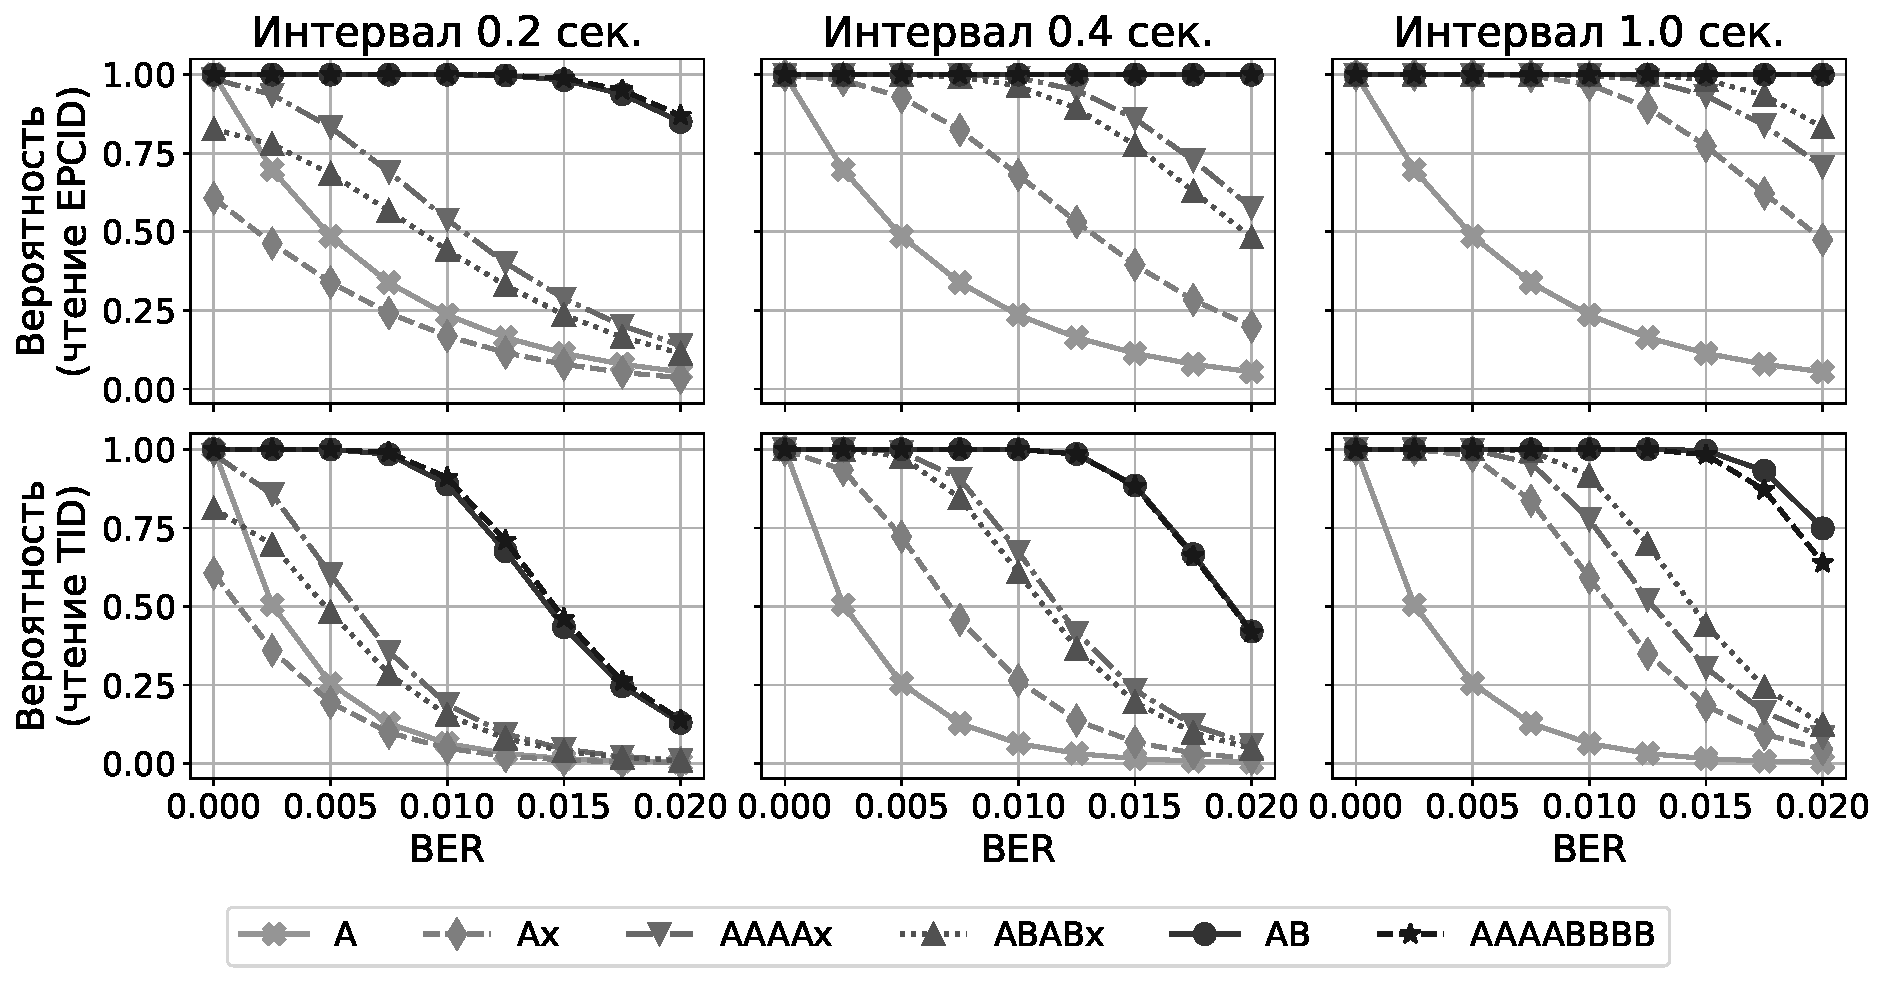
\includegraphics[scale=0.4]{chapter3/ch3_results_probs.pdf}
  }
  \caption{Вероятность успешной идентификации в разных сценариях работы считывателя при различных интервалах между метками. Метка находится в области чтения 2,5~сек.}\label{fig:id_prob_var_scenario}
\end{figure}

Численные результаты, полученные с помощью аналитической модели, представлены в \S~6 главы 3. Показано, что периодические сбросы питания и смены флагов опроса ведут к значительному увеличению вероятности успешной идентификации даже при высоких значениях BER, см. рис.~\ref{fig:id_prob_var_scenario}. Для валидации аналитической модели, результаты расчета сравнивались с данными имитационного моделирования.


% Можно сослаться на свои работы в автореферате. Для этого в файле
% \verb!Synopsis/setup.tex! необходимо присвоить положительное значение
% счётчику \verb!\setcounter{usefootcite}{1}!. В таком случае ссылки на
% работы других авторов будут подстрочными.
% Изложенные в третьей главе результаты опубликованы в~\cite{vakbib1, vakbib2}.
% Использование подстрочных ссылок внутри таблиц может вызывать проблемы.

%------------------------------------------------------------------------------
% ГЛАВА 4 (ТМО)
%------------------------------------------------------------------------------
\textbf{Четвертая глава}
посвящена исследованию производительности многошаговых опорных беспроводных сетей с помощью сетей массового обслуживания с узлами типа MAP/PH/1/N, а также быстрым методам вычисления характеристик многофазных сетей массового обслуживания. В \S~1 вводится объект исследования (многошаговая беспроводная сеть) и модель (многофазная система массового обслуживания) и ставится формальная задача исследования производительности сети с точки зрения оценки межконцевых задержек $T$ и вероятностей потерь пакетов $P_l$.

В \S~2 более подробно рассматривается модель "--- многофазная система массового обслуживания с марковскими входными потоками (MAP), распределениями времени обслуживания фазового типа (PH) и конечными очередями. Приводятся основные утверждения относительно систем MAP/PH/1/N и многофазных сетей, необходимые для расчета их характеристик. После этого приводится схема итерационного точного расчета средних межконцевых задержек $T$ и вероятностей потерь пакетов $P_l$. Приводится утверждение, показывающее экспоненциальный рост сложности расчета при увеличении числа узлов сети.

Для получения численных оценок характеристик открытой сети массового обслуживания в \S~3 приводится описание метода Монте-Карло и реализующей его дискретно-событийной имитационной модели сети массового обслуживания. Основной недостаток метода состоит в том, что для получения статистически устойчивых результатов необходимо моделировать большое число пакетов. Для того, чтобы сделать расчет характеристик более быстрым, можно использовать другой подход, основанный на аппроксимации потоков, передаваемых в сети. В \S~4 подробно рассматривается четыре различных подхода к аппроксимации потоков обслуженных пакетов, основанных на методе моментов:
\begin{enumerate}
  \item Аппроксимация по среднему $m_1$ пуассоновским потоком;
  \item Аппроксимация по среднему $m_1$ и коэффициенту варианции $c$ с помощью экспоненциальных и гиперэкспоненциальных распределений и распределения Эрланга;
  \item Аппроксимация PH-распределениями по среднему $m_1$ и коэффициентам вариации $c$ и ассимметрии $\gamma$ с помощью методов, предложенных в работе Johnson и Taafe,\autocite{Johnson1989}, а также в работе Telek и Heindl\autocite{Telek2003};
  \item Аппроксимация MAP-потоком по $m_1$, $c$, $\gamma$ и коэффициенту корреляции $\rho_1$ с помощью метода \autocite{Horvath2005} независимого поиска матрицы $D_1$ по найденному PH-распределению и коэффициенту корреляции.
\end{enumerate}

В \S~5 главы 4 предлагается методика построения тандемной сети массового обслуживания, моделирующей многошаговую беспроводную сеть проивзольного размера. На моделируемую сеть накладывается ряд ограничений: работа на одной частоте, видимость только непосредственных соседей, использование схемы доступа IEEE 802.11 DCF. Для нахождения распределений времени обслуживания предлагается использовать калибровочную беспроводную сеть с пятью станциями, для которой можно получить выборку интервалов передачи пакетов каждой из станций с помощью имитационной модели. При моделировании беспроводной сети произвольного размера для промежуточных каналов предлагается использовать PH-распределения, полученные для канала $S_2 \rightarrow S_3$ калибровочной сети.

Результаты численного исследования методов вычисления оценок характеристик многофазных сетей массового обслуживания с аппроксимацией выходящих потоков подробно изложены в \S~6 главы 4. Для оценки точности методов были сгенерированы 2500 случайных сетей. Для тех сетей, порядок выходящего потока с последней фазы в которых был достаточно мал, было найдено точное решение, для всех остальных "--- только приближенные оценки. Для каждого типа аппроксимаций рассматривалось два варианта применения: аппроксимация выходящих потоков и аппроксимация входящих потоков. Результаты сравнения точности методов показаны на рис.~\ref{fig:approximations_summary}. Хотя наиболее точные результаты показывает метод Монте-Карло, достаточно точные оценки (в пределах 10\%) удается найти с помощью аппроксимаций по трем моментам, а для нахождения оценок межконцевых задержек можно использовать даже аппроксимации по двум моментам, причем эти методы работают быстрее, чем метод Монте-Карло.

\begin{figure}[h]
  \centerfloat{
    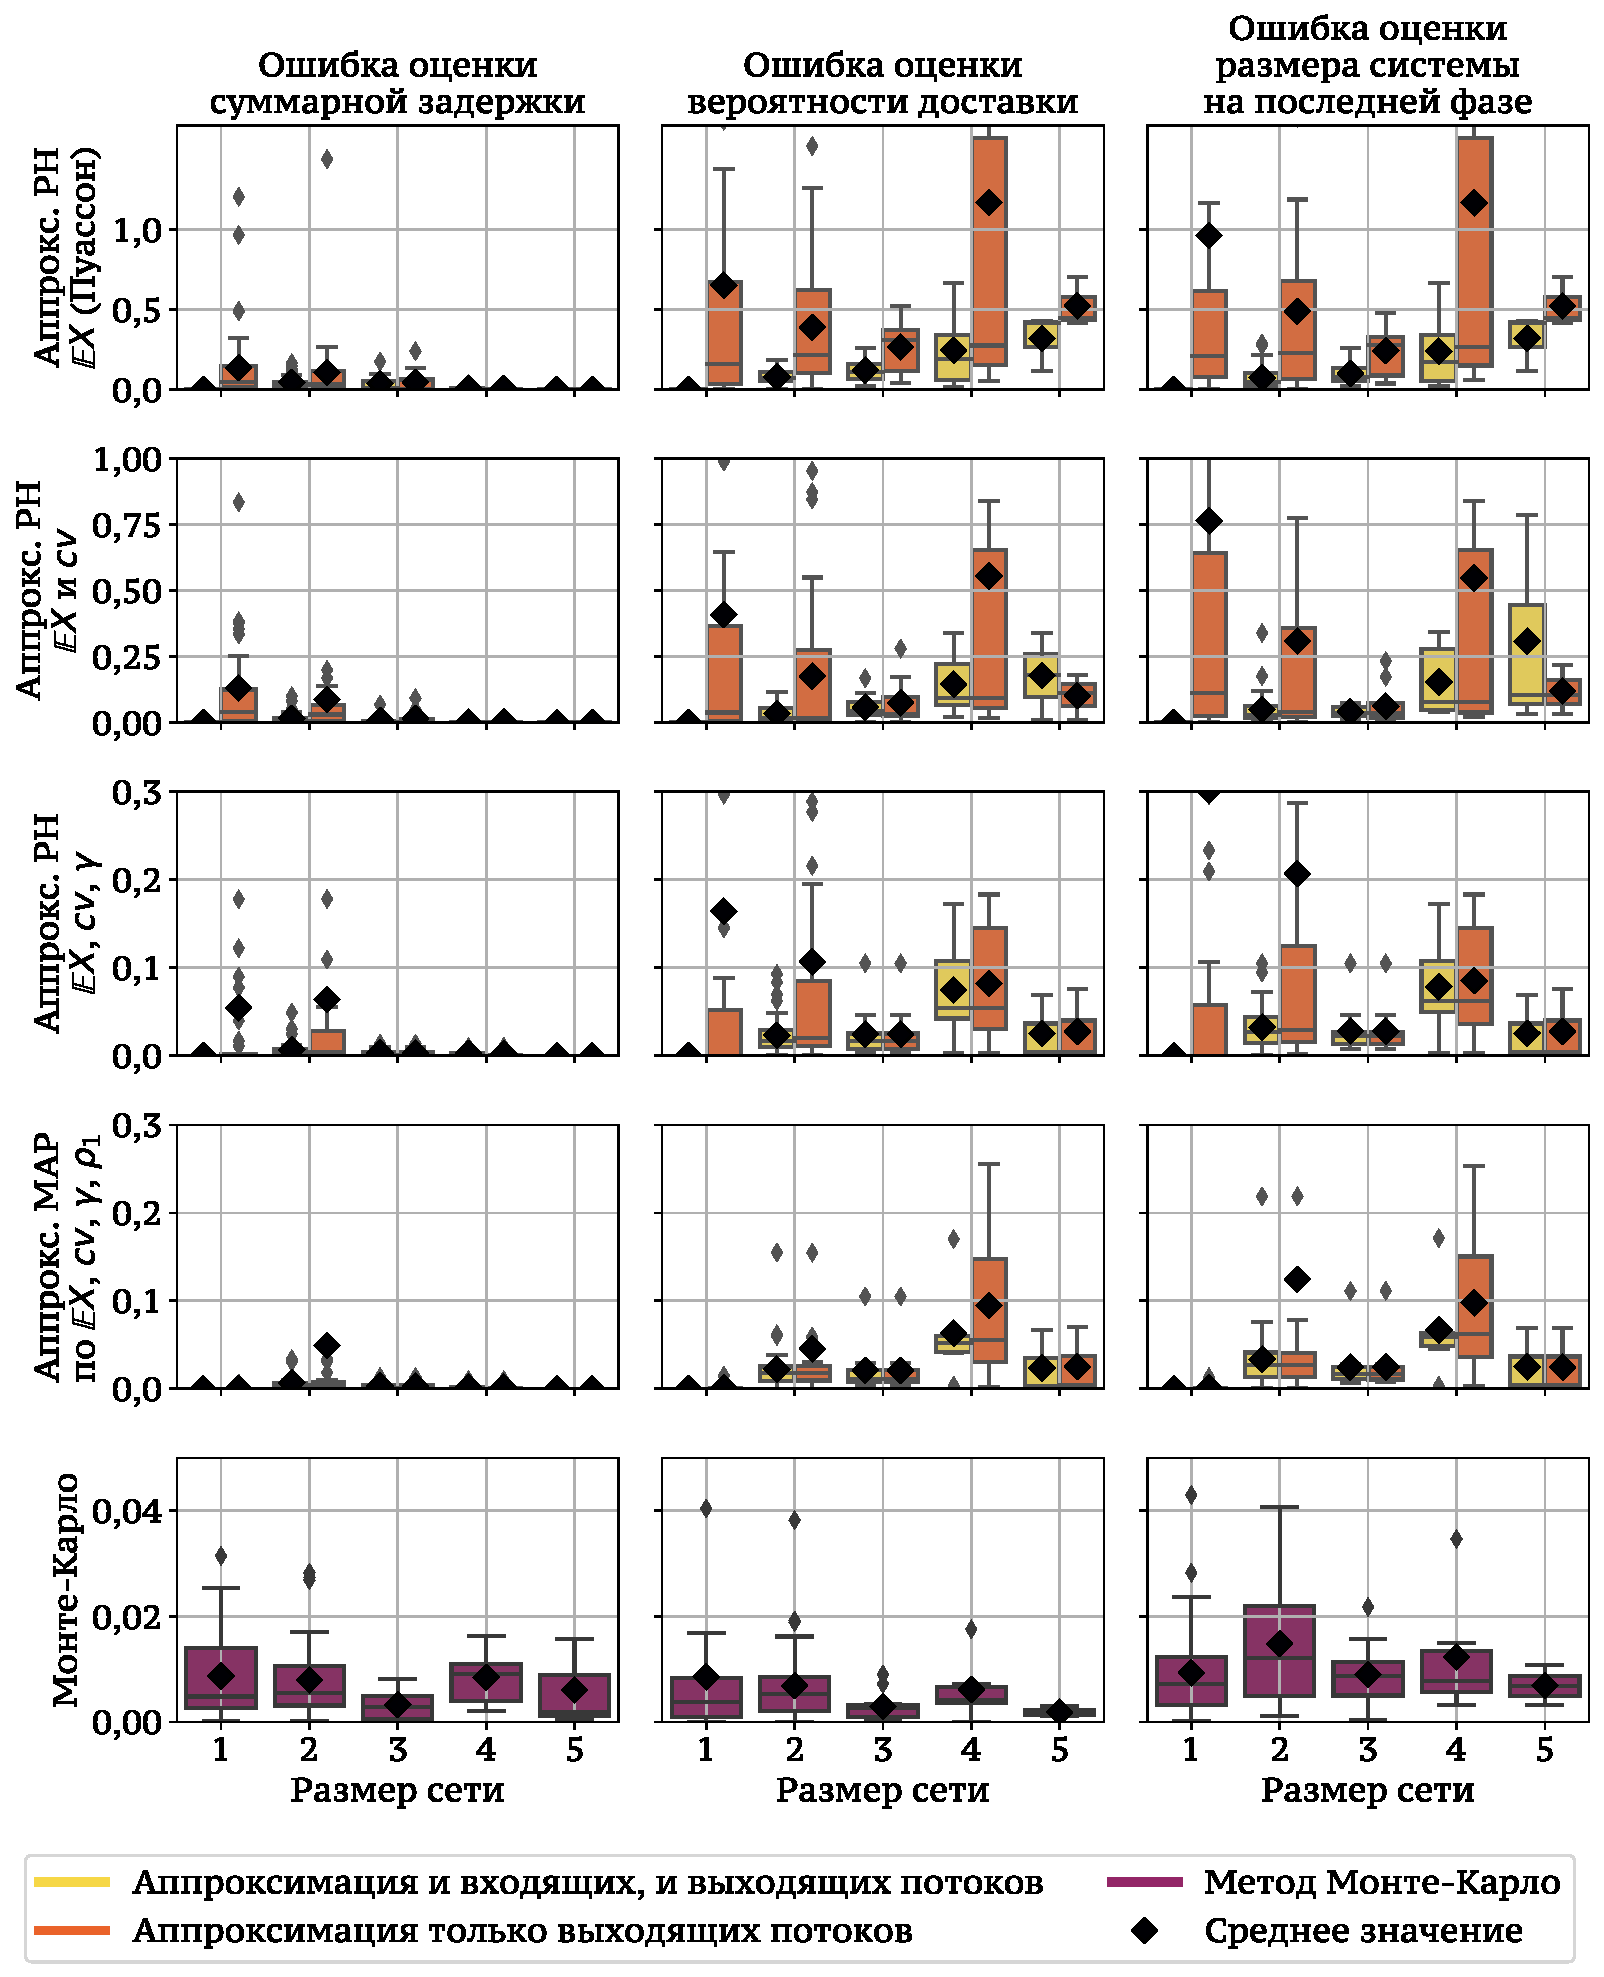
\includegraphics[scale=0.4]{chapter4/ch4_approximations_summary.pdf}
  }
  \caption{Точность оценок, полученных с помощью методов аппроксимаций потоков и метода Монте-Карло}
  \label{fig:approximations_summary}
\end{figure}

В \S~7 главы 4 приведены результаты численного исследования метода моделирования многошаговых беспроводных сетей с помощью сетей массового обслуживания, где распределения времени обслуживания вычисляются с помощью калибровочной сети. Входящий трафик моделировался с помощью пуассоновских потоков разных интенсивностей от 1,2 до 12 мегабит/с, а каналы беспроводной сети работали на скорости 56 мегабит/с по протоколу IEEE 802.11 DCF. Для моделирования беспроводной сети использовалась система моделирования NS-3. Распределения времени передачи в каналах моделировались с помощью PH-распределений, построенных по трем моментам, а также с помощью элементарных экспоненциальных распределений.

\begin{figure}[h]
  \centerfloat{
    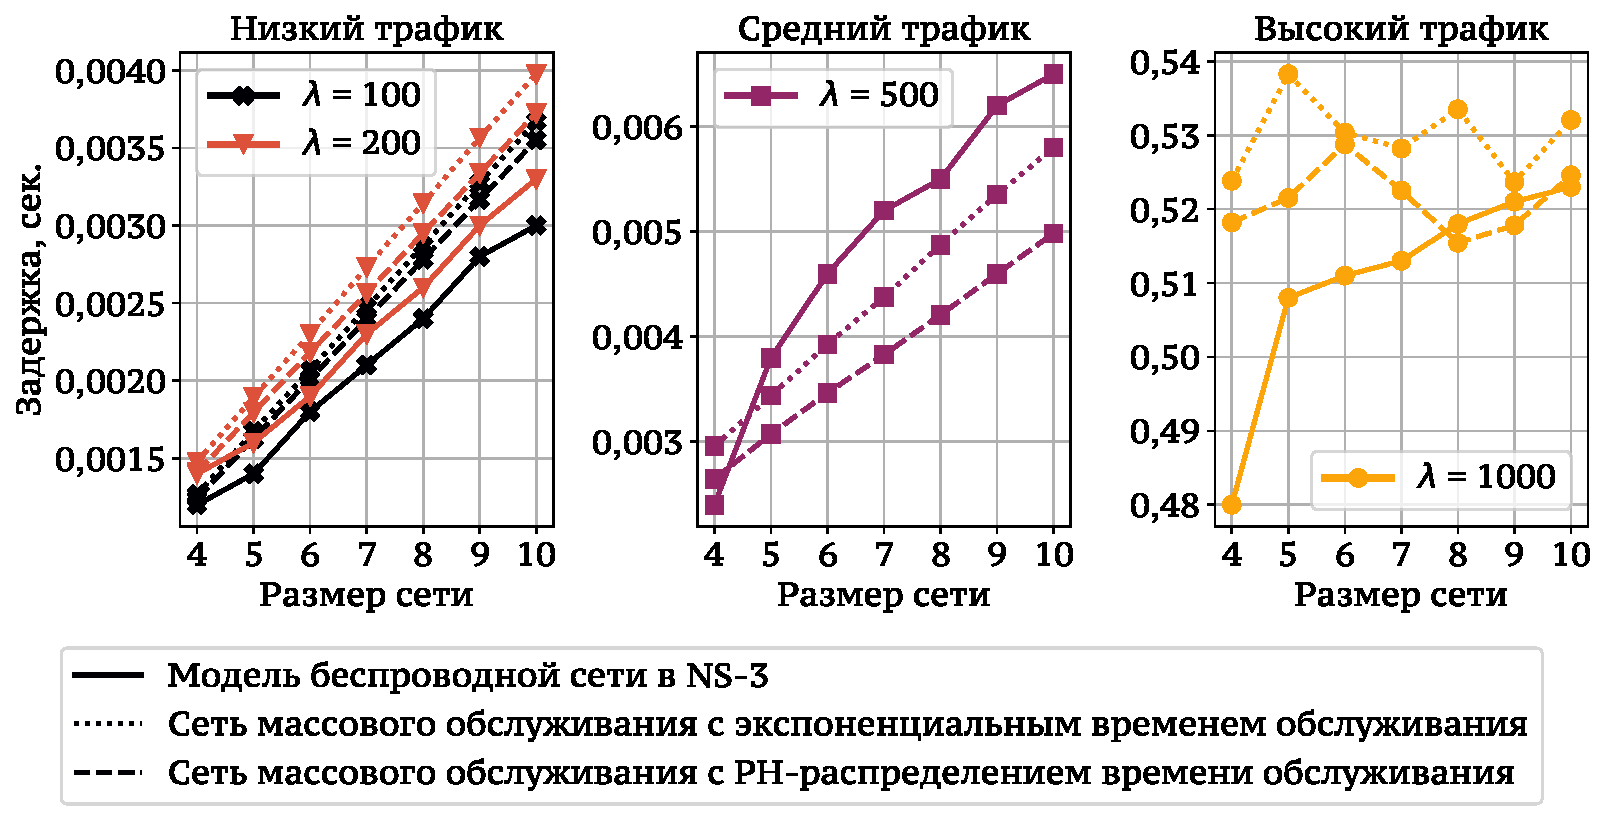
\includegraphics[scale=0.4]{chapter4/ch4_ns3_tandem_delays_refined.pdf}
  }
  \caption{Межконцевые задержки в сетях с каналами IEEE 802.11}\label{fig:tandem_delays}
\end{figure}

В ходе численного исследования было обнаружено, что в первых каналах беспроводной сети происходит существенная фильтрация трафика (потеря части пакетов), из-за чего задержки в каналах, расположенных ближе к источнику, оказываются существенно выше, чем в каналах, расположенных дальше. Для повышения точности моделирования было предложено изменить схему выбора распределений времени обслуживания: первые четыре канала моделировать с помощью распределений, полученных из калибровочной сети, а для времени обслуживания последующих каналов использовать распределение времени в последнем канале калибровочной сети. Обновленная методика позволила существенно увеличить точность оценки (в 1,4 -- 5 раз), особенно при высокой нагрузке в сети. На рис.~\ref{fig:tandem_delays} показаны результаты вычисления межконцевых задержек, полученные с помощью имитационной модели беспроводной сети в NS-3 и с помощью построенных по обновленной методике сетей массового обслуживания.



%------------------------------------------------------------------------------
% ГЛАВА 5 (ВНЕДРЕНИЕ)
%------------------------------------------------------------------------------
В \textbf{главе 5}
приведено описание разработанной автором распределенной системы управления RFID-считывателями и представлены результаты проведенных экспериментов по внедрению системы радиочастотной идентификации в 2014, 2020 и 2021 годах в городе Казань и на ЦКАД. В \S~1 главы 5 приведена архитектура системы управления считывателями, кратко описаны основные программные компоненты и приведены различные способы их размещения.

Протоколы связи между компонентами подробно описаны в \S~2. Протокол IMMP (Internal Modules Management Protocol) используется для управления и настройки компонентов со стороны центрального компонента (супервайзера), протокол SUAP (Simple User Access Protocol) используется для передачи команд управления от пользовательских интерфейсов, протокол ITOP (Internal Tag-Operation Protocol) используется для управления компонентами, работающими с RFID-модулями, а протокол TFP (Tag Flow Protocol) используется для подключения внешних пользователей к системе и получения ими потоков считанных меток.  В \S~3 приведено детальное описание компонентов системы: супервайзера, RFID-адаптера, сервера TFP и утилиты UAX, используемой для подключения пользовательских интерфейсов. Описаны принципы их работы и организаиця параллельной обработки запросов, в частности "--- способ мультиплексирования команд управления и чтения меток в RFID-адаптерах. \S~4 посвящен описанию реализации RFID-считывателя, а также программной реализации системы управления на языках C/C++.

В \S~5 главы 5 приведено описание эксперимента 2014 года, в ходе которого разработанными RFID-считывателями было оборудовано две точки идентификации, а в центре обработки данных ГИБДД был размещен сервер, в котором собирались данные о прочитанных метках. Сами метки были установлены в автомобильные номера и ими были осноащены 920 автобусов. Эксперимент продолжался три зимних месяца, с декабря по февраль, в результате была получена вероятность успешной идентификации 92~\% и 95~\%. В ходе эксперимента были выявлены проблемы с перегруженной видеонаблюдением сетью, которые были решены добавлением кэширования на считывателях, но свидетельствуют о целесообразности построения недорогих выделенных беспроводных сетей для подключения считывателей. В \S~6 описаны результаты протокольных испытаний, проведенный на полигоне в городе Казань, в которых изучалась эффективность радиочастотной идентификации при проезде автомобилей на скоростях до 150~км/ч, а также при различных маневрах "--- следовании, обгоне. RFID-метки, разработанные ПАО <<Микрон>>, были установлены в автомобильные номера. Во всех экспериментах все автомобили были успешно идентифицированы. Эксперимент по внедрению RFID на ЦКАД в 2021 году описан в \S~7.


%------------------------------------------------------------------------------
% ЗАКЛЮЧЕНИЕ
%------------------------------------------------------------------------------
\FloatBarrier
\pdfbookmark{Заключение}{conclusion}                                  % Закладка pdf
В \textbf{заключении} приведены основные результаты работы, которые заключаются в следующем:
%% Согласно ГОСТ Р 7.0.11-2011:
%% 5.3.3 В заключении диссертации излагают итоги выполненного исследования, рекомендации, перспективы дальнейшей разработки темы.
%% 9.2.3 В заключении автореферата диссертации излагают итоги данного исследования, рекомендации и перспективы дальнейшей разработки темы.
\begin{enumerate}
  \item Описан способ построения распределенной системы радиочастотной идентификации автомобилей, выделены факторы, влияющие на производительность системы.
  \item Представлены результаты численного исследования аналитической модели UHF RFID, показывающие целесообразность периодической смены считывателем опрашиваемого значения флага сессии и периодического сброса питания.
  \item Предложена имитационная модель системы радиочастотной идентификации автомобилей, учитывающая особенности распространения сигнала вблизи дороги, эффект Доплера, параметры антенных систем, настройки протокола EPC Class 1 Gen.2.
  \item С помощью имитационного моделирования получены численные оценки вероятности идентификации быстро движущихся автомобилей при различных настройках протокола. Полученные результаты показывают, что возможно добиться высокой вероятности идентификации при размещении меток в номерных знаках.
  \item Предложена методика построения открытых сетей массового обслуживания с узлами MAP/PH/1/N, адекватно моделирующих многошаговые беспроводные сети с каналами IEEE 802.11. Для обеспечения высокой точности модели, при поиске распределений времени обслуживания используются данные имитационного моделирования беспроводных каналов связи. Предложенная методика обеспечивает точность свыше 80~\% при многократном увеличении скорости расчета.
  \item Предложен метод приближенного расчёта характеристик тандемных сетей массового обслуживания с узлами MAP/PH/1/N,   позволяющий ограничить пространство состояний модели за счет использования методов аппроксимации выходящих MAP-потоков. Аппроксимация производится PH-распределениями по 1, 2 или 3 моментам, а также MAP-потоками по трем моментам и коэффициенту корреляции. Аппроксимация PH-распределениями по трем моментам позволяет с высокой точностью получить оценки характеристик сетей с большим числом узлов, требуя меньше времени, чем метод Монте-Карло.
  \item Предложена архитектура распределенной системы управления и промежуточного программного обеспечения для подключения RFID-считывателей к центру управления, обеспечивающего получение данных от считывателей, мониторинг и управление системой.
  \item Представлены результаты экспериментов по исследованию и внедрению системы радиочастотной иденификации автобусов в городе Казань 2014 и 2020 годов, а также в Московской области в 2021 году. Показано, что эффективность системы достигает 95~\%.
\end{enumerate}


\pdfbookmark{Литература}{bibliography}                                % Закладка pdf
% При использовании пакета \verb!biblatex! список публикаций автора по теме
% диссертации формируется в разделе <<\publications>>\ файла
% \verb!common/characteristic.tex!  при помощи команды \verb!\nocite!

\ifdefmacro{\microtypesetup}{\microtypesetup{protrusion=false}}{} % не рекомендуется применять пакет микротипографики к автоматически генерируемому списку литературы
\urlstyle{rm}                               % ссылки URL обычным шрифтом
\ifnumequal{\value{bibliosel}}{0}{% Встроенная реализация с загрузкой файла через движок bibtex8
  \renewcommand{\bibname}{\large \bibtitleauthor}
  \nocite{*}
  \insertbiblioauthor           % Подключаем Bib-базы
  %\insertbiblioexternal   % !!! bibtex не умеет работать с несколькими библиографиями !!!
}{% Реализация пакетом biblatex через движок biber
  % Цитирования.
  %  * Порядок перечисления определяет порядок в библиографии (только внутри подраздела, если `\insertbiblioauthorgrouped`).
  %  * Если не соблюдать порядок "как для \printbibliography", нумерация в `\insertbiblioauthor` будет кривой.
  %  * Если цитировать каждый источник отдельной командой --- найти некоторые ошибки будет проще.
  %
  %% authorvak
  \nocite{WINET_TCOMM2015}
  \nocite{QS_JPU2013}
  \nocite{QS_JITCS2013}
  \nocite{QS_TCOMM2012}

  %% authorwos - journals

  \nocite{QS_MDPI2021}
  \nocite{RFID_JRFID2017}
  \nocite{WINET_IJPAM2016}

  % \nocite{vakbib1}%
  % \nocite{vakbib2}%
  %
  %% authorwos
  % \nocite{wosbib1}%
  \nocite{QS_ICAAPSP2020}
  \nocite{QS_ITMM2019}
  \nocite{RFID_IEEERFID2018}
  \nocite{RFID_SYNCHROINFO2018}
  \nocite{RFID_IEEERFID2017}
  \nocite{QS_AICT2017}
  \nocite{QS_ITMM2017}
  \nocite{QS_ITMM2016}
  \nocite{QS_DCCN2016_CCIS}
  \nocite{RFID_DCCN2016_CCIS}
  \nocite{RFIDCTRL_NETS2CARS2014}
  \nocite{RFIDTA2012}

  %
  %% authorscopus
  % \nocite{scbib1}%
  %
  %% authorpathent
  % \nocite{patbib1}%
  %
  %% authorprogram
  % \nocite{progbib1}%
  %
  %% authorconf
  % \nocite{confbib1}%
  % \nocite{confbib2}%
  %
  %% authorother
  % \nocite{bib1}%
  % \nocite{bib2}%

  \ifnumgreater{\value{usefootcite}}{0}{
    \begin{refcontext}[labelprefix={}]
      \ifnum \value{bibgrouped}>0
        \insertbiblioauthorgrouped    % Вывод всех работ автора, сгруппированных по источникам
      \else
        \insertbiblioauthor      % Вывод всех работ автора
      \fi
    \end{refcontext}
  }{
  \ifnum \totvalue{citeexternal}>0
    \begin{refcontext}[labelprefix=A]
      \ifnum \value{bibgrouped}>0
        \insertbiblioauthorgrouped    % Вывод всех работ автора, сгруппированных по источникам
      \else
        \insertbiblioauthor      % Вывод всех работ автора
      \fi
    \end{refcontext}
  \else
    \ifnum \value{bibgrouped}>0
      \insertbiblioauthorgrouped    % Вывод всех работ автора, сгруппированных по источникам
    \else
      \insertbiblioauthor      % Вывод всех работ автора
    \fi
  \fi
  %  \insertbiblioauthorimportant  % Вывод наиболее значимых работ автора (определяется в файле characteristic во второй section)
  \begin{refcontext}[labelprefix={}]
      \insertbiblioexternal            % Вывод списка литературы, на которую ссылались в тексте автореферата
  \end{refcontext}
  % Невидимый библиографический список для подсчёта количества внешних публикаций
  % Используется, чтобы убрать приставку "А" у работ автора, если в автореферате нет
  % цитирований внешних источников.
  \printbibliography[heading=nobibheading, section=0, env=countexternal, keyword=biblioexternal, resetnumbers=true]%
  }
}
\ifdefmacro{\microtypesetup}{\microtypesetup{protrusion=true}}{}
\urlstyle{tt}                               % возвращаем установки шрифта ссылок URL
